\iffalse
\documentclass[journal,12pt,onecolumn]{IEEEtran}
\usepackage{cite}
\usepackage{amsmath,amssymb,amsfonts,amsthm}
\usepackage{algorithmic}
\usepackage{graphicx}
\usepackage{textcomp}
\usepackage{xcolor}
\usepackage{txfonts}
\usepackage{listings}
\usepackage{enumitem}
\usepackage{mathtools}
\usepackage{gensymb}
\usepackage{comment}
\usepackage[breaklinks=true]{hyperref}
\usepackage{tkz-euclide}
\usepackage{braket}
\def\inputGnumericTable{}
\usepackage[latin1]{inputenc}
\usepackage{color}
\usepackage{array}
\usepackage{longtable}
\usepackage{calc}
\usepackage{multirow}
\usepackage{hhline}
\usepackage{ifthen}
\usepackage{lscape}
\usepackage{gvv} 
\usepackage{circuitikz}

\newtheorem{theorem}{Theorem}[section]
\newtheorem{problem}{Problem}
\newtheorem{proposition}{Proposition}[section]
\newtheorem{lemma}{Lemma}[section]
\newtheorem{corollary}[theorem]{Corollary}
\newtheorem{example}{Example}[section]
\newtheorem{definition}[problem]{Definition}
\newcommand{\BEQA}{\begin{eqnarray}}
\newcommand{\EEQA}{\end{eqnarray}}
\newcommand{\define}{\stackrel{\triangle}{=}}
\theoremstyle{remark}
\newtheorem{rem}{Remark}
\renewcommand{\brak}[1]{\left(#1\right)}
\begin{document}

\bibliographystyle{IEEEtran}
\vspace{3cm}

\title{GATE 2021 CH-36}
\author{EE23BTECH11201 - Abburi Tanusha$^{*}$% <-this % stops a space
}
\maketitle

\renewcommand{\thefigure}{\theenumi}
\renewcommand{\thetable}{\theenumi}

\vspace{3cm}

\maketitle
\textbf{Question:} 
For the ordinary differential equation
\begin{align*}
\frac{d^3y}{dt^3} + 6\frac{d^2y}{dt^2} + 11\frac{dy}{dt} + 6y = 1,
\end{align*}
with initial conditions $y(0) = y'(0) = y''(0) = y'''(0) = 0$, the value of 
\begin{align*}
\lim_{{t \to \infty}} y(t) &= ?
\end{align*}
(round off to $3$ decimal places).
\hfill(GATE CH 2021)\\
\textbf{Solution:}
\fi
\begin{table}[h]
 	\centering
 	\resizebox{6 cm}{!}{
 		
\begin{tabular}{|c|c|l|}
\hline
Parameter  & Value & Description   \\             
\hline
$y(0)$     & $0$   & Initial displacement  \\     
 \hline
$y'(0)$    & $0$   & First derivative at $t=0$  \\
 \hline
$y''(0)$   & $0$   & Second derivative at $t=0$ \\
 \hline
$y'''(0)$  & $0$   & Third derivative at $t=0$  \\
 \hline
\end{tabular}


 	}
 	\vspace{6 pt}
 	\caption{Parameters}
 \end{table}
\begin{align}
\frac{d^3y}{dt^3} + 6\frac{d^2y}{dt^2} + 11\frac{dy}{dt} + 6y &= 1
\end{align}
Applying the Laplace transform to both sides:
\begin{align}
s^3Y(s) + 6s^2Y(s) + 11sY(s) + 6Y(s) &= \frac{1}{s} \\
Y(s)\brak{s^3 + 6s^2 + 11s + 6} &= \frac{1}{s} \\
\implies Y(s) &= \frac{1}{s\brak{s+1}\brak{s+2}\brak{s+3}} ; \quad Re(s) > 0
\end{align}
\begin{align}
Y(s) &= \frac{A}{s} + \frac{B}{s+1} + \frac{C}{s+2} + \frac{D}{s+3} \\
1 &= A\brak{s+1}\brak{s+2}\brak{s+3} + Bs\brak{s+2}\brak{s+3} + Cs\brak{s+1}\brak{s+3} + Ds\brak{s+1}\brak{s+2}  \\
1 &= A\brak{s^3 + 6s^2 + 11s + 6} + Bs\brak{s^2 + 5s + 6}  + Cs\brak{s^2 + 4s + 3} + Ds\brak{s^2 + 3s + 2} \\
\end{align}
Comparing the coefficients on both sides \\
\begin{align}
A + B + C + D = 0 \\
6A + 5B + 4C + 3D = 0 \\
11A + 6B + 3C + 2D = 0 \\
6A = 1 \\
A=1/6 ,B = -11/26 , C= 5/26 , D= 5/78 
\end{align}
Substitute these values 
\begin{align}
Y(s) = \frac{6}{s} - \frac{11}{26\brak{s+1}} + \frac{5}{26\brak{s+2}} + \frac{5}{78\brak{s+3}}
\end{align}
Apply Inverse Laplace Transform 
\begin{align}
y(t) &= 6\mathcal{L}^{-1}\brak{\frac{1}{s}} - 11\mathcal{L}^{-1}\brak{\frac{1}{26\brak{s+1}}} + 5\mathcal{L}^{-1}\brak{\frac{1}{26\brak{s+2}}} + 5\mathcal{L}^{-1}\brak{\frac{1}{78\brak{s+3}}} \\
y(t) &= 6 - \frac{11}{26}e^{-t} + \frac{5}{26}e^{-2t} +\frac{5}{78}e^{-3t}
\end{align}
Consider
\begin{align}
\lim_{t \to \infty} y(t) &= \lim_{t \to \infty} \brak{6 - \frac{11}{26}e^{-t} + \frac{5}{26}e^{-2t} +\frac{5}{78}e^{-3t}} \\
&= 6
\end{align}\
Verifying using Final Value Theorem :\\
\begin{align}
 \lim_{t \to \infty} y(t)   &= \lim_{s \to 0} sY(s)  \\
\lim_{s \to 0} sY(s) &= \lim_{s \to 0} s \brak{ \frac{6}{s} - \frac{11}{26\brak{s+1}} + \frac{5}{26\brak{s+2}} + \frac{5}{78\brak{s+3}}} \\
&= \lim_{s \to 0} \brak{ 6 - \frac{11s}{26\brak{s+1}} + \frac{5s}{26\brak{s+2}} + \frac{5s}{78\brak{s+3}}} \\
&= 6
\end{align}

\begin{figure}[h!]
\centering
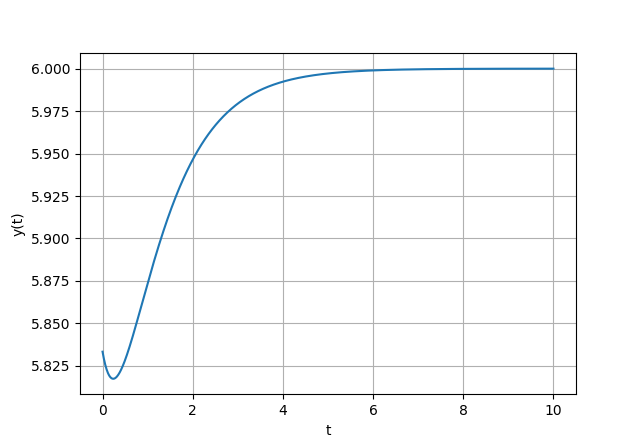
\includegraphics[width=\columnwidth]{2022/CH/36/figs/plot.png}
\caption{Plot $y(t)$ vs $t$ }
\end{figure}
%\end{document}
